\begin{frame}
  \begin{center}
    {
      \huge GloVe: Global Vectors for Word Representation
    } \\
    Pennington,Socher,Manning
  \end{center}
\end{frame}
%%%%%%%%%%%%%%%%%%%%%%%%%%%%%%%%%%%%%%%%%%%%%%%%%%

\begin{frame}{Introduction - What is a Word Vector?}
  \begin{itemize}
    %% Word vectors capture linguistic regularities in a simple manner.
  \item A mathematical representation of words.
    %% conventional way - one hot repr lead to data sparsity, does not take word relationships into account
  \item Representation captures some form of ``related-ness''.
    \begin{figure}
      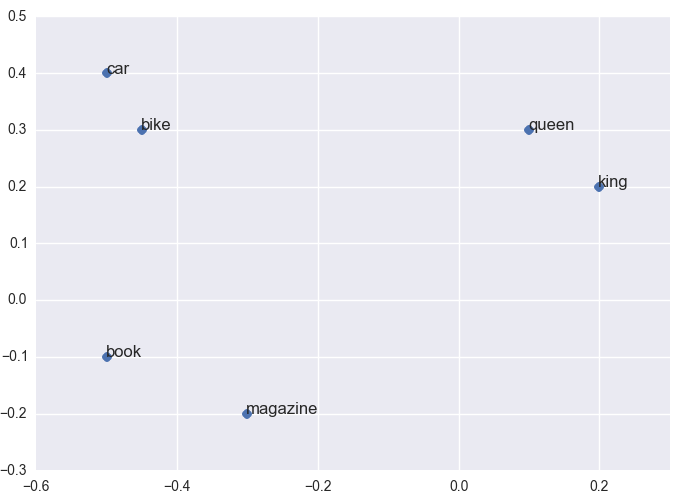
\includegraphics[scale=0.35]{images/wordvec.png}
      \caption{From}
    \end{figure}    
  \end{itemize}
\end{frame}


%%%%%%%%%%%%%%%%%%%%%%%%%%%%%%%%%%%%%%%%%%%%%%%%%%
\begin{frame}{Generating Vector Representations}
  Word vectors can be generated in the following ways:
  \begin{itemize}[<+->]
  \item Cooccurence Matrix Factorization~\cite{Deerwester} % HAL,LSA the name of the game is compute co-occurence
    % fully unsupervised!
  \item Learn representation from Local Context ~\cite{Mikolov13a}.%
  \item Sometimes just using the explicit context representation suffices ~\cite{Levy14}.
    %% Sometimes these methods end-up modeling the same objective (skip-gram).
    %% what abt random sampling
  \end{itemize}
  %% Say its task specific, therefore there has been a explosion of papers on this topic.
  %% \visible<4>{
  %%   This paper proposes another way of obtaining word vectors via matrix factorization.
  %% }
  %% They claim that their model combines advantages of both global and local? (??)
\end{frame}

%%%%%%%%%%%%%%%%%%%%%%%%%%%%%%%%%%%%%%%%%%%%%%%%%%
\begin{frame}{Structure in Word Vector Spaces}
  The configuration of the vectors encode relationships between words.
  \begin{align*}
    vec(king) - vec(man) + vec(woman) \approx vec(queen)
  \end{align*}
  \pause
  \visible<2->{
    \begin{figure}
      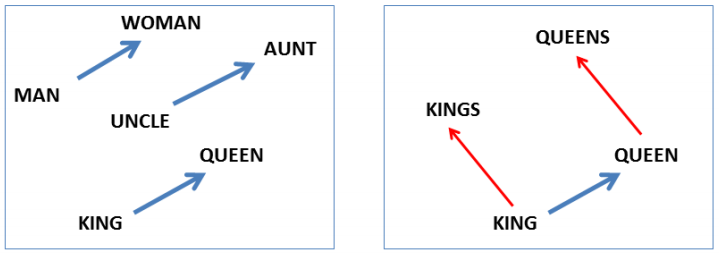
\includegraphics[scale=0.35]{images/mikolov.png}
      \caption{From}
    \end{figure}
  }
  %% No explanation was given in the original papers.
  %% {\footnotesize Remarkably, training such a lexical model induces word repr. with striking semantic and syntactic properties---\cite{Mikolov13a}} \\
  %% Levy showed that tranditional methods like count sparse contexts can perform equally well.
  %% {\footnotesize ... traditional word similarities can perform just as well as neural embeddings ---\cite{Levy14}} \\
  %% talk about Dont Count Predict paper
  \visible<3>{
    This paper claims to explicitly model the properties needed for achieving the above effect.
  }
\end{frame}

%%   Global Matrix Factorization Methods are prone to ill-effects of predominance of function words.
%%   They claim their objective is explicitly modelling vector structure to facilitate linear 

%%%%%%%%%%%%%%%%%%%%%%%%%%%%%%%%%%%%%%%%%%%%%%%%%%
\begin{frame}{GloVe Model - Intuition}
  \begin{figure}
    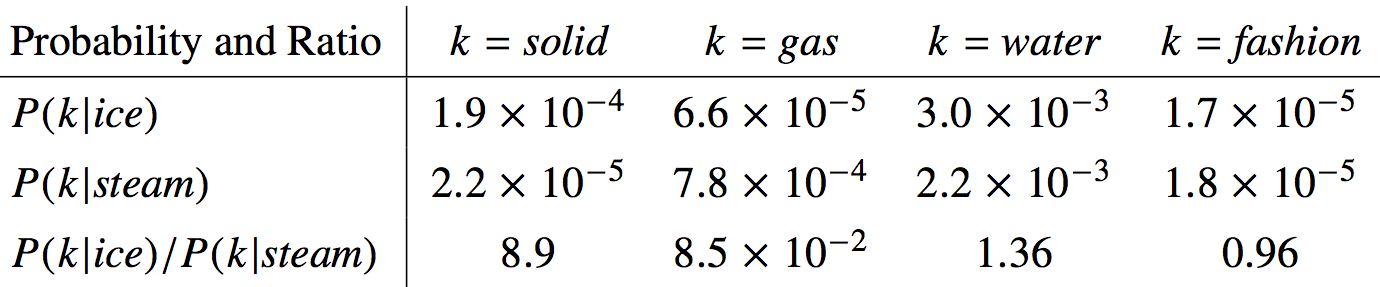
\includegraphics[scale=0.23]{images/glove_int.png}
  \end{figure}
  \visible<2>{
    \begin{align*}
      \frac{\Pr(k \mid king)}{\Pr(k \mid queen)} \approx \frac{\Pr(k \mid man)}{\Pr(k \mid woman)} \Forall k
    \end{align*}    
  }
\end{frame}

%%%%%%%%%%%%%%%%%%%%%%%%%%%%%%%%%%%%%%%%%%%%%%%%%%
\begin{frame}{GloVe Model - Derivation of Objective}
  \begin{align*}
    %% & \Pr(\text{word j appears in context of word i}) = \Pr_{ij} \\
    \visible<1->{& \Pr_{ij} \propto \exp({w_i}^T{\tilde{w}_j}) \tag{log-bilinear model} \\}
    \visible<2->{& w_i^T\tilde{w_j} + \tilde{b_j} = \log X_{ij} - \log X_{i} \tag{$\Pr_{ik}=\frac{X_{ik}}{X_i}$} \\}
    %% & \frac{\Pr_{ik}}{\Pr_{jk}}=\exp(\dotprod{w_i -w_j}{\tilde{w}_k}) \\
    %% & \log \Pr_{ik} - \log\Pr_{jk} = \dotprod{w_i -w_j}{\tilde{w}_k}\\
    \visible<3->{& w_i^T\tilde{w_j} +b_i + \tilde{b_j} = \log X_{ij}}
  \end{align*}
  \visible<4->{
    We can minimize 
    \begin{align*}
      & \sum_{i=1,j=1}^V \left( w_i^T\tilde{w_j} +b_i + \tilde{b_j} - \log X_{ij} \right)^2
    \end{align*}
  }
  %% note the similarity with matrix factorization
  \begin{center}
    \visible<5->{But wait!}
  \end{center}
\end{frame}

%%%%%%%%%%%%%%%%%%%%%%%%%%%%%%%%%%%%%%%%%%%%%%%%%%
\begin{frame}{GloVe Model - Introduce Weighted Cost}
  \begin{align*}
    & J = \sum_{i=1,j=1}^V \alert{f(X_{ij})} \left( w_i^T\tilde{w_j} +b_i + \tilde{b_j} - \log X_{ij} \right)^2
  \end{align*}
  \begin{center}
    $f$ should not overweight rare and too-frequent occurences.
  \end{center}
  \visible<2->{
    \begin{align*}
      f(x)=
      \begin{cases}
        (x/x_{max})^\alpha & \text{ if $x < x_{max}$} \\
        1 & \text{ otherwise}
      \end{cases}
      %% explain what x_max and \alpha do
    \end{align*}
  }
  \visible<3->{
    \begin{figure}
      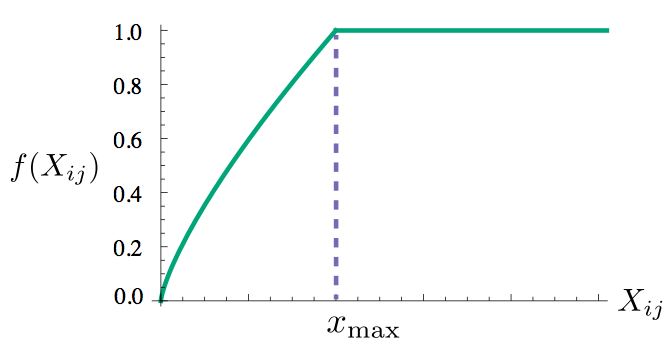
\includegraphics[scale=0.27]{images/weighting.png}
      \caption{From}
    \end{figure}
  }
\end{frame}

%%%%%%%%%%%%%%%%%%%%%%%%%%%%%%%%%%%%%%%%%%%%%%%%%%
%% \begin{frame}{Model Parameters and Training}
%%   \begin{itemize}
%%   \item $x_{max},\alpha$
%%   \item window size, vector dimension
%%   \item corpus size
%%   \end{itemize}
%%   \begin{itemize}[<+->]
%%   \item Compute $X$
%%   \item $J$ is optimized using SGD.
%%   \end{itemize}
%% \end{frame}

%%%%%%%%%%%%%%%%%%%%%%%%%%%%%%%%%%%%%%%%%%%%%%%%%%
%% \begin{frame}{Model Analysis}
%%   \begin{itemize}
%%   \item Vector Length:
%%   \item Context Size: 
%%   \item Corpus Size: nothing suprising
%%   \item Model trained on smaller wikipedia corpus( 1.6B tokens) does better on semantic task than model trained on larger corpus like gigaword (4.3B tokens)
%%   \item Idea: instead of using only word vector $w$, use $w+c$, where $c$ is the context vector (significant improvement in semantic task). This can be used for other models as well.
%%   \end{itemize}
%% \end{frame}

%%%%%%%%%%%%%%%%%%%%%%%%%%%%%%%%%%%%%%%%%%%%%%%%%%
\begin{frame}{Training and Evaluation}

  \begin{exampleblock}{Training}
    \begin{itemize}[<+->]
    \item Compute matrix $X$
    \item Do SGD.
    \end{itemize}
  \end{exampleblock}
  
  \onslide<3->
  \begin{exampleblock}{Evaluation}
    \begin{itemize}[<+->]
    \item Semantic Relatedness % (Google Dataset) % intrinsic
      \begin{itemize}
      \item \textsc{Athens} is to \textsc{Greece} as \textsc{Berlin} is to ? (\textsc{Germany})
      \item \textsc{Putin} is to \textsc{Russia} as \textsc{Sarkozy} is to ? (\textsc{France})
      \end{itemize}
    \item Syntactic Relatedness % (Google dataset, MSR dataset) % intrinsic
      \begin{itemize}
      \item \textsc{Car} is to \textsc{Cars} as \textsc{Family} is to ? (\textsc{families})
      \item \textsc{Carry} is to \textsc{Carried} as \textsc{Go} is to ? (\textsc{went})
      \end{itemize}
    \item NER 
      \begin{itemize}
      \item Uses word vectors as continuous features in a NER system.
      \end{itemize}
    \end{itemize}
  \end{exampleblock}
\end{frame}

%%%%%%%%%%%%%%%%%%%%%%%%%%%%%%%%%%%%%%%%%%%%%%%%%%
\begin{frame}{Results on Analogy Discovery}
  %% \begin{figure}
  %%   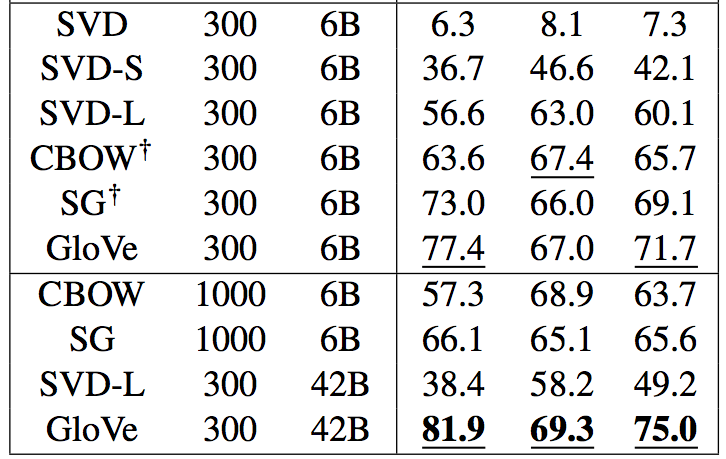
\includegraphics[scale=0.27]{images/results1_1.png}
  %% \end{figure}
  \begin{figure}
    \centering
    \begin{tabular}{|ccc|ccc|}
      \hline
      Model & Dim. & Size & Sem. & Syn. & Tot.\\
      \hline
      SVD & 300 & 6B & 6.3 & 8.1 & 7.3\\
      SVD-S & 300 & 6B & 36.7 & 46.6 & 42.1\\
      SVD-L & 300 & 6B & 56.6 & 63.0 & 60.1\\
      CBOW & 300 & 6B & 63.6 & 67.4 & 65.7\\
      SG & 300 & 6B & 73.0 & 66.0 & 69.1\\
      GloVe & 300 & 6B & 77.4 & 67.0 & 71.7\\
      \hline
      CBOW & 1000 & 6B & 57.3 & 68.9 & 63.7\\
      SG & 1000 & 6B & 66.1 & 65.1 & 65.6\\
      SVD-L & 300 & 6B & 38.4 & 58.2 & 49.2\\
      GloVe & 300 & 6B & 81.9 & 69.3 & 75.0\\
      \hline
    \end{tabular}
    \caption{\% accuracy on analogy discovery}
  \end{figure}
\end{frame}

%%%%%%%%%%%%%%%%%%%%%%%%%%%%%%%%%%%%%%%%%%%%%%%%%%
\begin{frame}{Results on Word Similarity}
  \begin{figure}
    %% 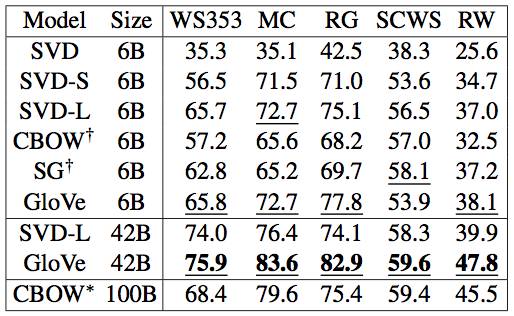
\includegraphics[scale=0.4]{images/results2.png}
    \begin{tabular}{|cc|ccccc|}
      \hline
      Model & Size & WS353 & MC & RG & SCWS & RW\\
      \hline
      SVD & 6B & 35.3 & 35.1 & 42.5 & 38.3 & 25.6 \\
      SVD-S & 6B & 56.5 & 71.5 & 71.0 & 53.6 & 34.7\\
      SVD-L & 6B & 65.7 & 63.0 & 60.1 & 56.5 & 37.0\\
      CBOW & 6B & 57.2 & 65.6 & 68.2 & 57.0 & 32.5\\
      SG & 6B & 62.8 & 65.2 & 69.1 & 58.1 & 37.2\\
      GloVe & 6B & 65.8 & 72.7 & 77.8 & 53.9 & 38.1\\
      \hline
      SVD-L & 42B & 74.0 & 76.4 & 74.1 & 58.3 & 39.9\\
      GloVe & 42B & 75.9 & 83.6 & 82.9 & 59.6 & 47.8\\
      \hline
      CBOW & 100B & 68.4 & 79.6 & 75.4 & 59.4 & 45.5\\
      \hline
    \end{tabular}
    \caption{Spearman's correlation on word similarity with 300 dim. vectors.}
  \end{figure}
\end{frame}

%%%%%%%%%%%%%%%%%%%%%%%%%%%%%%%%%%%%%%%%%%%%%%%%%%
\begin{frame}{Results on NER}
  \begin{figure}
    %% 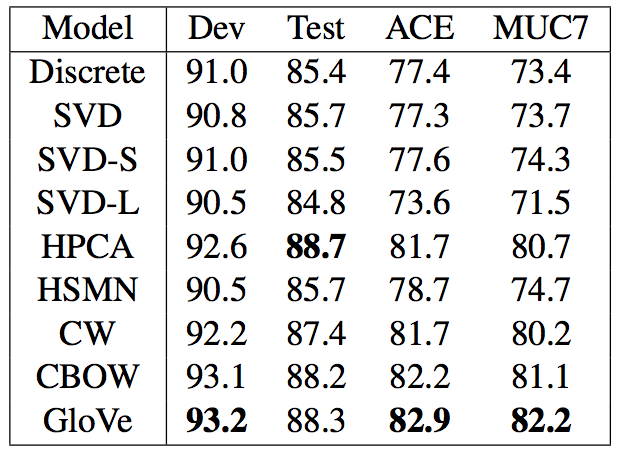
\includegraphics[scale=0.4]{images/ner.png}
    \begin{tabular}{|c|cccc|}
      \hline
      Model & Dev & Test & ACE & MUC7 \\
      \hline
      Discrete & 91.0 & 85.4 & 77.4 & 73.4\\
      SVD & 90.8 & 85.7 & 77.3 & 73.7\\
      SVD-S & 91.0 & 85.5 & 77.6 & 74.3\\
      SVD-L & 90.5 & 84.8 & 73.6 & 71.5\\
      HPCA & 92.6 & 88.7 & 81.7 & 80.7 \\
      CW & 92.2 & 87.4 & 81.7 & 80.2\\
      CBOW & 93.1 & 88.2 & 82.2 & 81.1\\
      GloVe & 93.2 & 88.3 & 82.9 & 82.2\\
      \hline
    \end{tabular}
    \caption{F1 on NER with 50d vectors.}
  \end{figure}
\end{frame}

%%%%%%%%%%%%%%%%%%%%%%%%%%%%%%%%%%%%%%%%%%%%%%%%%%
\begin{frame}{GloVe vs. word2vec}
  \begin{figure}
    \centering
    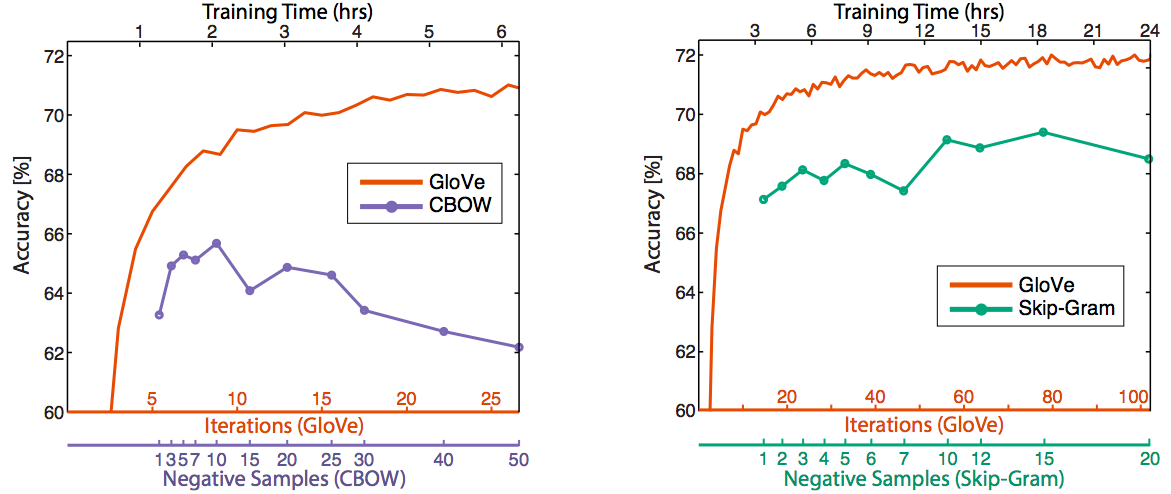
\includegraphics[scale=0.29]{images/gloveVSword2vec.png}
    \caption{Runtime and Accuracy Comparison}
    %% take this with a pinch of salt
  \end{figure}
\end{frame}

%%%%%%%%%%%%%%%%%%%%%%%%%%%%%%%%%%%%%%%%%%%%%%%%%%
\begin{frame}{Choice of Corpus}
  \begin{figure}
    \centering
    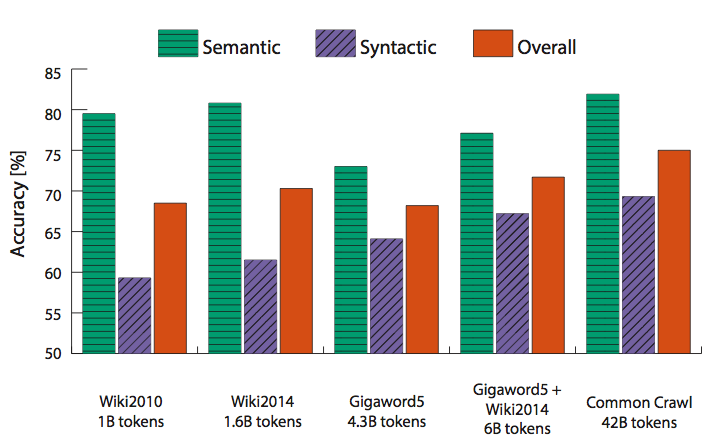
\includegraphics[scale=0.4]{images/corpus.png}
    %% \begin{subfigure}[b]{0.33\textwidth}
    %%   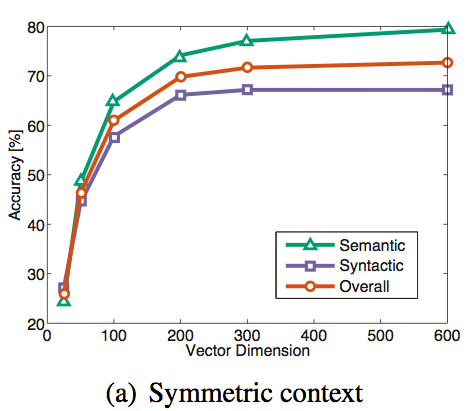
\includegraphics[width=\textwidth]{images/analogy1.png}
    %% \end{subfigure}%
    %% \begin{subfigure}[b]{0.33\textwidth}
    %%   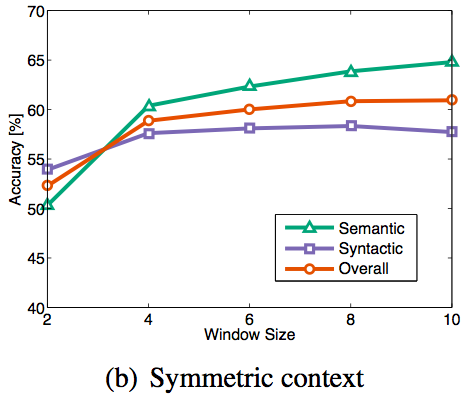
\includegraphics[width=\textwidth]{images/analogy2.png}
    %% \end{subfigure}%
    %% \begin{subfigure}[b]{0.33\textwidth}
    %%   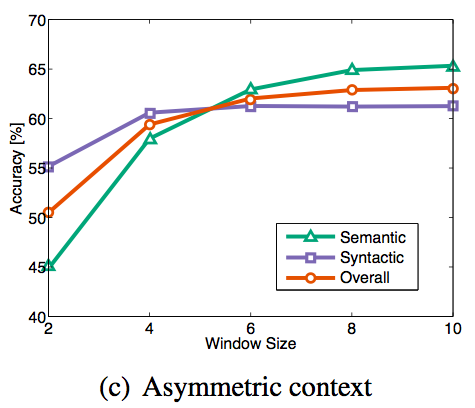
\includegraphics[width=\textwidth]{images/analogy3.png}
    %% \end{subfigure}%
  \end{figure}
\end{frame}

%%%%%%%%%%%%%%%%%%%%%%%%%%%%%%%%%%%%%%%%%%%%%%%%%%
\begin{frame}{Conclusion}
  \begin{itemize}
  \item Nice formulation
  \item 
  \item Missing 
  \end{itemize}
  new ideas from Turian Ratinov Bengio,
  curriculum training strategy?
  liang's preprocessing
  connotation vs denotation
  distributional vs distributed
  exp not done MSR dataset,
  batch restriction for glove vs online training for skip gram
\end{frame}
